\documentclass[11pt]{report}
%\documentclass{fmetfm}
%\documentclass{fmetfm}
\usepackage{amsbsy}
\usepackage{url}
\usepackage{amssymb}
\usepackage{amsmath}
\usepackage{amsfonts}
\usepackage{amsthm}
\usepackage{times}
\usepackage{appendix}
\usepackage{indentfirst}
\usepackage{graphicx}
\usepackage{subfig}
\usepackage[a4paper]{geometry}
%\usepackage{graphicx}
\usepackage[english]{babel}
\usepackage[utf8]{inputenc} 
\usepackage[colorlinks=true,linkcolor=black,citecolor=black,urlcolor=black]{hyperref}
\usepackage{tikz}
%\usepackage[square,numbers]{natbib}
\usepackage{chicago}
\usepackage{caption}
\usepackage{float}
\usepackage[nottoc]{tocbibind}
\usepackage{algorithm2e}
\SetKwComment{Comment}{$\triangleright$\ }{}
\usepackage{longtable}
%\usepackage{lipsum} % just for dummy text- not needed for a longtable
%\usepackage{multirow}
\usetikzlibrary{shapes,arrows}
\DeclareMathOperator{\Tr}{Trace}
\DeclareMathOperator{\diag}{diag}
\DeclareMathOperator{\range}{range}
\DeclareMathOperator{\cummds}{cum-mds}
\DeclareMathOperator{\eigen}{eigen}
\usepackage{Sweave}
\begin{document}
%%%   PORTADA  %%%

\begin{titlepage}
  \begin{center}
	  \textsf{\scshape\LARGE Universitat Politècnica de Catalunya\\[0.5em]
	          Facultat de Matemàtiques i Estadística}\vskip 8em
	  {\LARGE Master thesis \par} \vskip 8em
	  {\bfseries \huge Multidimensional Scaling for Big Data} \vskip 1.5em 
	  {\LARGE \lineskip .5em Cristian Pachón García \par} 
    \vskip 12em {\large Advisor: Pedro Delicado Useros \hskip 0.3em}
    \vfill {\large Dept. d'Estadística i Investigació Operativa }
  \end{center}
  \par
  \vskip 3.5em 
\end{titlepage}

\thispagestyle{empty}

%\begin{titlepage}
%\begin{center}
%\emph{}\\ [3cm]
%\rule{\textwidth}{2.5pt}
%\huge{\textbf{This is the tittle}}
%\rule{\textwidth}{2.5pt} \\ [6 cm]
%\large{Student: Cristian Pachon Garcia}\\[0.5 cm]
%\large{Director: Pedro Delicado}\\ [2.2 cm]
%\large{Master Thesis} \\ [0.3 cm]
%\large{(MESIO UPC-UB)} \\ [1.5 cm]
%\large{January 2019}
%\end{center}
%\end{titlepage}

\textwidth=6in
\textheight=9.2in
\oddsidemargin=0.3in
\evensidemargin=0.2in
\headheight=0.1in
\topmargin=-0.1in

\newcommand{\Robject}[1]{\texttt{#1}}
\newcommand{\Rpackage}[1]{\textsf{#1}}
\newcommand{\Rclass}[1]{\textit{#1}}
\newcommand{\R}{\textsf{R}}
\newcommand*{\h}{\hspace{5pt}}
\newcommand*{\hh}{\h\h}




%%%%%%%%%%%%%%%%%%%%%%%%

\setcounter{page}{1}



%\title{This is the tittle}
%\vspace{1cm}

%\author{Student: 
%Cristian Pachon Garcia\\
%\texttt{cc.pachon@gmail.com}
%\and
%Director: Pedro Delicado\\
%\texttt{pedroemail@upc.edu}
%}





%\date{January 2019} 
%\title{How hard would it be to build a spaceship from scrap}
%\author{Carl Capybara\thanks{I never procrastinate} \and Walter Wombat}
%\subtitle{A closer look at the expenses}
%\subject{a funny paper}




\thispagestyle{empty}



\Sconcordance{concordance:thesis.tex:thesis.Rnw:%
1 65 1 1 0 2720 1}


%\maketitle

\clearpage



\tableofcontents



\chapter{Classical Multidimensional Scaling}
\section{Introduction to Multidimensional Scaling}
Multidimensional Scaling (MDS) is a family of methods that represents 
measurements of dissimilarity (or similarity) among pairs of objects as 
Euclidean distances between points of a low-dimensional space. The data, 
for example, may be correlations among intelligence tests and the MDS 
representation is a plane that shows the tests as points. The graphical display 
of the correlations provided by MDS enables the data analyst to literally 
``look" at the data and to explore their structure visually. This often shows 
regularities that remain hidden when studying arrays of numbers. 

\indent Given a square matrix \textbf{D} $n\times n$, the goal of MDS is to 
obtain a configuration matrix \textbf{X} $n \times p$ with orthogonal columns
that can be interpreted as the matrix of $p$ variables for the $n$ 
observations, where the Eucliden distance between the rows of \textbf{X} 
is approximately equat to \textbf{D}. The columns of \textbf{X} are called 
\textit{principal coordinates}.

\indent This approach arises two questions: is it (always) possible to find this
low dimensional configuration \textbf{X}? How is it obtained? In general, it 
is not possible to find a set of $p$ variables that reproduces 
\textit{exactly} the initial distance. However, it is possible to find a set 
of variables which distance is approximately the initial distance matrix 
\textbf{D}.


\indent As classical example, consider the distances between European cities as
in the Table (\ref{european_distances}). One would like to get a representation in
a 2-dimensional space such that the distances would be almost the same as in the 
Table (\ref{european_distances}). The representation of these coordinates are 
displayed in Figure (\ref{europ_cities}).

\begin{table}[ht]
\centering
\begin{tabular}{rrrrrrr}
  \hline
 & Athens & Barcelona & Brussels & Calais & Cherbourg & $\dotsi$ \\ 
  \hline
Athens & 0 & 3313 & 2963 & 3175 & 3339 & $\dotsi$ \\ 
  Barcelona & 3313 & 0& 1318 & 1326 & 1294 & $\dotsi$ \\ 
  Brussels & 2963 & 1318 & 0 & 204 & 583 & $\dotsi$ \\ 
  Calais & 3175 & 1326 & 204 & 0 & 460 & $\dotsi$ \\ 
  Cherbourg & 3339 & 1294 & 583 & 460 & 0 & $\dotsi$ \\
  $\vdots$ & $\vdots$ & $\vdots$ & $\vdots$ & $\vdots$ & $\vdots$ & $\ddots$ \\
   \hline
\end{tabular}
\caption{Distances between European cities (just 5 of them are shown).} 
\label{european_distances}
\end{table}


\begin{figure}[ht]
\centering
    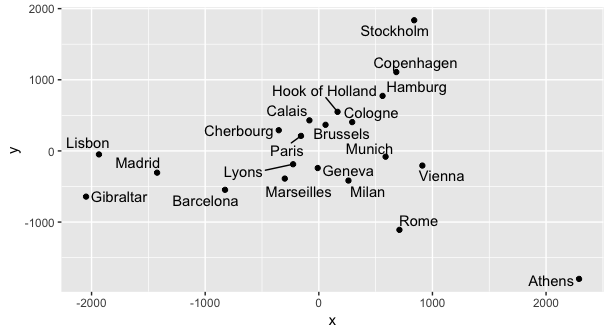
\includegraphics[scale = 0.5]{./images/europ_cities.png}
    \caption{MDS on the Eurepean cities.}
    \label{europ_cities}
\end{figure}

%\indent MDS methods can be divided into two groups: \textit{Metric MDS} and
%\textit{Non-metric MDS}. Metric MDS, also known as \texit{Principal Coordinates Analysis}, 
%uses the differences between similarities. However, Non-metric MDS states that if $a$
%is more similar to $b$ than $c$, then $a$ is closer to $b$ than $c$, but the
%differences between the similarities $ab$ and $ac$ do not have any 
%interpretation. This thesis is focused on the Metric MDS.

\section{Principal coordinates}
Given a matrix \textbf{X} $n \times p$, the matrix of $n$ 
individuals over $p$ variables, it is possible to obtain a new one with 
mean equal to 0 by column from the previous one:

\[
\mathbf{\widetilde{X}} = \Big( \mathbf{I} - \frac{1}{n} \mathbf{1}\mathbf{1'}\Big) \mathbf{X} = \mathbf{P}\mathbf{X},
\]
where 

\[
\mathbf{P} = \Big( \mathbf{I} - \frac{1}{n} \mathbf{1}\mathbf{1'}\Big).
\]

\indent This new matrix, $\mathbf{\widetilde{X}}$, has the same dimensions as 
the orginial one but its columns mean is \textbf{0}. From this matrix, it is 
possible to build two square semi-positive definite matrices: the covariance 
matrix \textbf{S}, defined as $\mathbf{\widetilde{X}'}\mathbf{\widetilde{X}}/n$ 
and the cross-prodructs matrix $Q = \mathbf{\widetilde{X}}\mathbf{\widetilde{X}'}$. 
The last matrix can be interpreted as a similarity matrix between the $n$ elements. 
The term $ij$ is obtained as follows:

\begin{equation} \label{qij}
q_{ij} = \sum_{s=1}^{p} x_{is}x_{js} = \mathbf{x_i'} \mathbf{x_j}
\end{equation}
where $\mathbf{x_i'}$ is the i-th row from $\mathbf{\widetilde{X}}$. 
Given the scalar product formula, ${\mathbf{x_i'}\mathbf{x_j} =  \mid \mathbf{x_i} \mid \mid \mathbf{x_i} \mid \cos\theta_{ij}}$,
if the elements $i$ and $j$ have similar coordinates, then $\cos\theta_{ij} \simeq 1$
and $q_{ij}$ will be large. On the contrary, if the elements are very different,
then $\cos \theta_{ij} \simeq 0$ and $q_{ij}$ will be small. So, 
$\mathbf{\widetilde{X}}\mathbf{\widetilde{X}'}$ can be interpreted as the similarity
matrix between the elements.

\indent The distances between elements can be deduced from the similarity 
matrix. The Eucliden distance between two elements is calculated in the 
following way:

\begin{equation} \label{dij}
d^2_{ij} =  \sum_{s=1}^{p} (x_{is}- x_{js} )^2  = \sum_{s=1}^{p}x_{is}^2 + \sum_{s=1}^p x_{js}^2 - 2\sum_{s=1}^{p} x_{is}x_{js}.
\end{equation}

\indent This expression can be obtained directly from the matrix \textbf{Q}:

\begin{equation} \label{dfromq}
d^2_{ij} = q_{ii} + q_{jj} - 2q_{ij}.
\end{equation}

\indent We have just seen that, given the matrix $\mathbf{\widetilde{X}}$, 
it is possible to get the similarity matrix 
$\mathbf{Q} = \mathbf{\widetilde{X}}\mathbf{\widetilde{X}'}$ and from it, 
to get the distance matrix \textbf{D}. Let $\diag(\mathbf{Q})$ be the
vector that contains the diagonal terms of \textbf{Q} and \textbf{1} be the vector
of ones, the matrix \textbf{D} is given by

\[
\mathbf{D} = \diag(\mathbf{Q}) \mathbf{1}' + \mathbf{1}\diag(\mathbf{Q})' - 2\mathbf{Q}.
\]

\indent The problem we are dealing with goes in the opposite direction. We want 
to rebuild $\mathbf{\widetilde{X}}$ from a square distance matrix \textbf{D}, 
with elements $d_{ij}^2$. The first step is to obtain \textbf{Q} and afterwards, 
to get $\mathbf{\widetilde{X}}$. The theory needed to get the solution can be 
found in \cite{pena_libro}. Here, we summarise it.

\indent The first step is to find out a way to obtain the matrix \textbf{Q} 
given \textbf{D}. We can assume without loss of generality that the mean of 
the variables is equal to 0. This is a consequence of the fact that the distance 
between two points remains the same if the variables are expressed in terms 
of the mean:


\begin{equation} \label{dtraslated}
d_{ij}^2 = \sum_{s = 1}^p (x_{is} - x_{js})^2 = \sum_{s=1} ^p [(x_{is} - \overline{x_s})- (x_{js} - \overline{x_s})]^2.
\end{equation}

\indent The previous condition means that we are lookig for a matrix  
$\mathbf{\widetilde{X}}$ such that $\mathbf{\widetilde{X}'}\mathbf{1} = 0$. 
It also means that $\mathbf{Q}\mathbf{1} = 0$, i.e, the sum of all the elements 
of a column of \textbf{Q} is 0. Since the matrix is symmetric, the previous 
condition should state for the rows as well. 

\indent To establish these constrains, we sum up (\ref{dfromq}) at row level:

\begin{equation} \label{sumrows}
\sum_{i = 1}^n d_{ij}^2 = \sum_{i = 1}^n q_{ii} + nq_{jj} = t + nq_{jj}
\end{equation}
where $t = \sum_{i = 1}^n q_{ii} = \Tr(\mathbf{Q})$, and we have used that the
condition \textbf{Q}\textbf{1} = 0 implies $\sum_{i = 1}^n q_{ij} = 0$. Summing 
up (\ref{dfromq}) at column level:

\begin{equation} \label{sumcols}
\sum_{j = 1}^n d_{ij}^2 = t + nq_{ii}.
\end{equation}

\indent Summing up (\ref{sumrows}) we obtain:

\begin{equation} \label{doublesum}
\sum_{i = 1}^n\sum_{j = 1}^n d_{ij}^2 = 2nt
\end{equation}

\indent Replacing in (\ref{dfromq}) $q_{jj}$ obtained in (\ref{sumrows}) and $q_{ii}$
obtained in (\ref{sumcols}), we have the following expression:

\begin{equation} \label{generaldij}
d_{ij}^2 = \frac{1}{n}\sum_{i = 1}^n d_{ij}^2 - \frac{t}{n} + \frac{1}{n} \sum_{j = 1}^n d_{ij}^2 -\frac{t}{n} -2q_{ij}
\end{equation}

\indent Let $d_{i.}^2 = \frac{1}{n}\sum_{j = 1}^n d_{ij}^2$ and $d_{.j}^2 = \frac{1}{n}\sum_{i=1}^n d_{ij}^2$ 
be the row-mean and column-mean of the elements of \textbf{D}. Using 
(\ref{doublesum}), we have that

\begin{equation} \label{dmeans}
d_{ij}^2 = d_{i.}^2 + d_{.j}^2 - d_{..}^2-2q_{ij}
\end{equation}
where $d_{..}$ is the mean of all the elements of \textbf{D}, given by

\[
d_{..}^2 = \frac{1}{n^2}\sum \sum d_{ij}^2.
\]

\indent Finally, from (\ref{dmeans}) we get the expression:

\begin{equation} \label{qij2}
q_{ij} = -\frac{1}{2}(d_{ij}^2 - d_{i.}^2 - d_{.j}^2 + d_{..}^2).
\end{equation}

\indent The previous expression shows how to build the matrix of similarities 
\textbf{Q} from the distance matrix \textbf{D}.

\indent The next step is to obtain the matrix \textbf{X} given the matrix 
\textbf{Q}. Let's assume that the similarity matrix is positive definite of 
range $p$. Therefore, it can be represented as

\[
\mathbf{Q} = \mathbf{V}\mathbf{\Lambda}\mathbf{V'}
\]
where $\mathbf{V}$ is a $n \times p$ matrix that contains the eigenvectors with
not nulls eigenvalues of \textbf{Q}. $\mathbf{\Lambda}$ is a diagonal matrix 
$p \times p$ that contains the eigenvalues.

\indent Re-writing the previous expression, we obtain

\begin{equation} \label{generalQ}
\mathbf{Q} = (\mathbf{V}\mathbf{\Lambda}^{1/2})(\mathbf{\Lambda}^{1/2}\mathbf{V'}).
\end{equation}

Getting

\[
\mathbf{Y} = \mathbf{V}\mathbf{\Lambda}^{1/2}.
\]

We have obtained a matrix with dimensions $n \times p$ with $p$ uncorrelated
variables that reproduce the initial metric. It is important to notice that if 
one starts from \textbf{X} (i.e \textbf{X} is known) and calculates from these
variables the distance matrix in (\ref{dij}) and after that it is applied
the method explained, the matrix obtained is not the same as \textbf{X}, but
its principal components. This happens since the distance between the rows in
a matrix does not change if:

\begin{itemize}
\item The row-mean values are modified by adding the same row vector to all
the rows in \textbf{X}.
\item Rows are rotated, i.e, \textbf{X} is postmultiplied by an orthogonal 
matrix.
\end{itemize}

\indent By (\ref{dfromq}), the distance is a function of the terms of the 
similarity matrix \textbf{Q} and this matrix is invariant given any rotation,
reflexion or translation of the variables

\[
\mathbf{Q} = \mathbf{\widetilde{X}} \mathbf{\widetilde{X'}} = \mathbf{\widetilde{X}} \mathbf{A} \mathbf{A'}\mathbf{\widetilde{X'}}
\]
for any orthogonal \textbf{A} matrix. The matrix \textbf{Q} only contains 
information about the space generated by the variables \textbf{X}. Any rotation,
reflexion or translation keeps the distance unchaged. Therefore, the solution
is not unique.


\section{Building principal coordinates}
%In general, the distance matrix is not compatible with an Eucliden metric but
%usually the similarity matrix obtained from it has $p$ positive eigenvalues  
%which are greater than the other ones. If the rest $n-p$ of not null eigenvalues 
%are much less than the other ones, it is possible to obtain an (approximated)
%representation using the $p$ eigenvectors associated with the first $p$
%eigenvalues of the similarity matrix. 

\indent Let \textbf{D} be a square distance matrix. The process to obtain 
the \textit{principal coordinates} is:

\begin{enumerate}
\item Build the matrix $\mathbf{Q = - \frac{1}{2} PDP}$ of cross-products.
\item Obtain the eigenvalues of \textbf{Q}. Take the $r$ greatest eigenvalues. 
Since $\mathbf{P1}=0$, where \textbf{1} is a vector of ones, 
$\range(\mathbf{Q})=n-1$, being the vector \textbf{1} an eigenvector with 
eigenvalue 0. 
\item Obtain the coordinates of the rows in the variables 
$\mathbf{v_i}\sqrt{\lambda_i}$,
where $\lambda_i$ is an eigenvalue of \textbf{Q} and $\mathbf{v_i}$ is the
associated unitary eigenvector. This implies that \textbf{Q} is apporximated by:

\[
\mathbf{Q} \approx (\mathbf{V_r \Lambda}^{1/2})(\mathbf{\Lambda_r}^{1/2} \mathbf{V_r'}).
\]

\item Take as coordinates of the points the following variables:
\[
\mathbf{Y_r} = \mathbf{V_r}\mathbf{\Lambda_r}^{1/2}.
\]
\end{enumerate}

\indent The method can also be applied if the initial information is not a 
distance matrix but a similarity matrix. A \textit{similarity function}, 
$s_{ij}$, between two element $i$ and $j$  is defined as:

\begin{itemize}
\item $s_{ii} = 1$.
\item $0 \leq s_{ij} \leq 1$.
\item $s_{ij} = s_{ji}$.
\end{itemize}

If the initial information is \textbf{Q}, a similariy matrix, then $q_{ii} = 1$,
$q_{ij} = q_{ji}$ and $0 \leq q_{ij} \leq 1$. The associated distance matrix 
is

\[
d_{ij}^2 = q_{ii} + q_{jj} - 2q_{qij} = 2(1-q_{ij}),
\]
and it is easy to see that $\sqrt{2(1-q_{ij})}$ is a distance and it verifies
the triangle inequality.


\section{Procrustes transformation}
As we have mentioned before, the MDS solution is not unique. One example of it 
is shown in Figure (\ref{twosol}).

\begin{figure}[ht]
    \centering
    \subfloat[]{{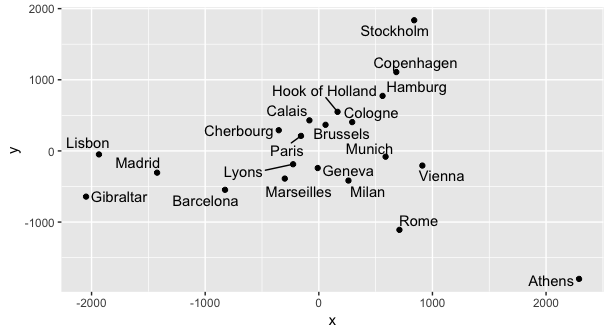
\includegraphics[width=8cm]{./images/europ_cities.png} }}%
    \qquad
    \subfloat[]{{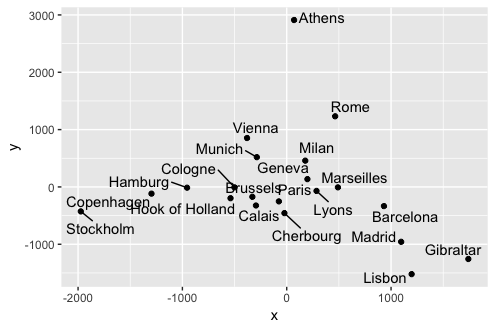
\includegraphics[width=8cm]{./images/europ_cities_rot.png} }}%
    \caption{Two different solutions of MDS.}%
    \label{twosol}%
\end{figure}


\indent Since rotations, translations and reflections are distance-preserving 
functions, one can find two different MDS configurations 
for the same set of data. How is it possible to align both solutions? This 
problem is solved by means of \textit{Procrustes transformations}.  


\indent The Procrustes problem is concern with fitting a configuration (testee)
to another (target) as closely as possible. In the simple case, both 
configurations have the same dimensionality and the same number of points, which
can be brought into 1-1 correspondence by substantive considerations. Under
orthogonal transformations, the testee can be fitted it to the target. In 
addition to such rigid motions, one may also allow for dilations and for shifts.

\indent All the details are developed in  \cite{BorgGroenen2005}. This is out 
of the scope of this thesis. However, since it has been a repeatdly used tool, 
we briefly summarise it. 

\indent Let \textbf{A} and \textbf{B} be two different MDS configurations for
the same set of data. Without loss of generality, let's assume that the target 
is \textbf{A} and the testee is \textbf{B}. One wants to obtain $s$, \textbf{T}
and \textit{t} such that

\[
\mathbf{A} = s \mathbf{B} \mathbf{T} + \mathbf{1t}'
\]
where \textbf{T} is an orthogonal matrix. As mentioned before, 
in \cite{BorgGroenen2005} are all the details needed to estimate 
these parameters.

\section{Multidimensional Scaling with \textsf{R}}

All the algorithms have been coded in \textsf{R}, since it has a widely 
statistics packages already implemented. We have used two packages for 
developing our MDS approaches:

\begin{itemize}
\item Package: \textsf{stats}. From this one we have used the function 
\textsf{cmdscale} to do the MDS. The output of this function is:
\begin{itemize}
\item The new coordinates for the individuals.
\item All the eigenvalues found.
\end{itemize}
\item Package: \textsf{MCMCpack}. From this one we have used the function 
\textsf{procrustes} to do the Procrustes transformation. The output of 
this function is:
\begin{itemize}
\item The dilation coeficient $s$.
\item The orthogonal matrix \textbf{T}.
\item The translation vector \textbf{t}.
\end{itemize}
\end{itemize}

\chapter{Algorithms for Multidimensional Scaling with Big Data}

\section{Why is it needed?}
In this chapter we present the algorithms developed so that MDS can be applied
when we are dealing with large datasets. The natural question here is why we need 
them if there are already some implementations. To answer this question, let's 
take a look at the Figures (\ref{elapsed_time_mds}) and (\ref{memory_distance}).

 
\begin{figure}[ht]
\centering
    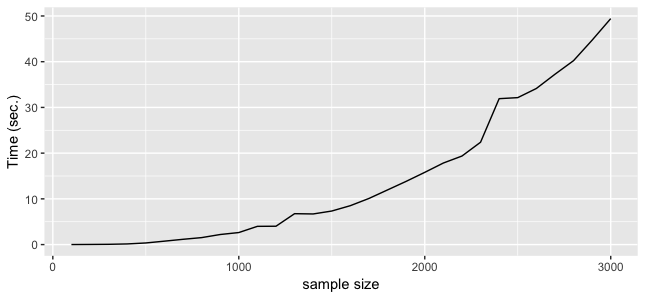
\includegraphics[scale = 0.5]{./images/elapsed_time_mds.png}
    \caption{Elapsed time to compute MDS.}
    \label{elapsed_time_mds}
\end{figure}



\begin{figure}[ht]
\centering
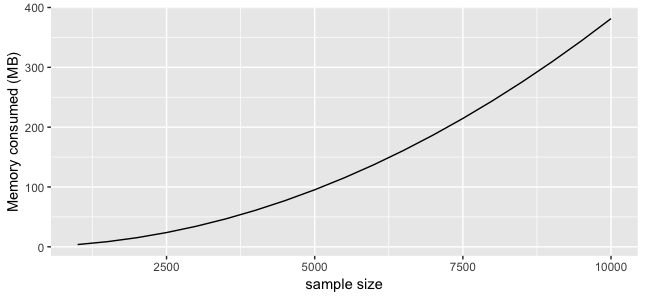
\includegraphics[scale = 0.5]{./images/memory_distance.png}
\caption{Memory consumed to compute distance.}
\label{memory_distance}
\end{figure}


\indent Figure (\ref{elapsed_time_mds}) shows the time needed to compute MDS
as a function of the sample size. As we can see, the time grows 
exponentially. Apart of the time issue, there is another one related to the
memory needed to compute the distance matrix. Figure (\ref{memory_distance}) 
points out that it is required at least 400MB to store the distance 
matrix when the dataset is close to 10000 observations.

\indent In order to solve these problems, we have developed three algorithms:


\begin{itemize}
\item \textit{Divide and Conquer MDS:} Before this thesis, 
\textit{Pedro Delicado} had done some work about  MDS with big
datasets and he had already created a first approach, which is this one. The 
algorithm is based on the idea of dividng and conquering. Given a big dataset, 
it is divided into $p$ partitions. After that, MDS is performed over all the 
partitions and, finally, the $p$ solutions are stitched so that all the points 
lie on the same coordinate system.

\item \textit{Fast MDS:} during the phase of gathering information, we found an 
article that solved the problem of scalability \cite{Yang06afast}. The 
authors  use a divide and conquer idea together with recursive programming. 

\item \textit{MDS based on Gower interpolation formula:} this algorithm uses
Gower interpolation formula which allows to add a new set of points
to an existing MDS configuration \cite{gowerformula}. 

\end{itemize}

In the next sections we provide a description of the algorithms. 
If further details about the implementation are needed, the code is provided in 
\autoref{chap:code}.

\section{Divde and Conquer Multidimensional Scaling}
\subsection{Algorithm}

\begin{itemize}

\item The first step is to divide the original dataset into $p$ partitions: 
$\mathbf{X_1},\dots, \mathbf{X_p}$. The number of partitions, $p$, is also
the number of steps needed to compute the algorithm.

\item Calculate the MDS for the first partition: \textbf{MDS(1)}. This solution
will be used as a guide to align the MDS for the remaining partitions. We 
use a new variable, \textbf{cum-mds}, that will be growing as long as new 
partitions are used. Before adding a new MDS, it is aligned and, after 
that, added. 

\item Define \textbf{cum-mds} equal to \textbf{MDS(1)} and start iterating 
until the last partition is reached.

\item Given a step $k$, $1 < k \leq p$, partitions $k$ and \textit{k-1} are 
joint, i.e, $\mathbf{X_k} \cup \mathbf{X_{k-1}}$. MDS is calculated on 
this union, obtaining $\mathbf{MDS_{k, k-1}}$. In order to add the
rows of the \textit{k-th} partition to \textbf{cum-mds}, the following steps 
are performed:

\begin{itemize}
\item Take the rows of the partition \textit{k-1} from $\mathbf{MDS_{k, k-1}}$: 
$\mathbf{MDS_{k, k-1}} \Bigr|_{k-1}$.
\item Take the rows of the partition \textit{k-1} from \textbf{cum-mds}: 
\textbf{cum-mds} $\Bigr|_{k-1}$.
\item Apply Procrustes to align both solutions. It means that a scalar number
\textit{s}, a vector \textbf{t} and an orthogonal matrix \textbf{T} are obtained
so that
\[
\boldsymbol{\cummds} \Bigr|_{k-1} = s \mathbf{MDS_{k, k-1}} \Bigr|_{k-1} \mathbf{T} + \mathbf{1t}'.
\]
\item Take the rows of the partition $k$ from $\mathbf{MDS_{k, k-1}}: \mathbf{MDS_{k, k-1}} \Bigr|_{k}$.
\item Use the previous Procrustes parameters to add the rows of 
$\mathbf{MDS_{k, k-1}} \Bigr|_{k}$ to \textbf{cum-mds}:
\[
\boldsymbol{\cummds}_k := s \mathbf{\mathbf{MDS_{k, k-1}}} \Bigr|_{k} \mathbf{T} + \mathbf{1t}'.
\]
\item Add the previous dataset to \textbf{cum-mds}, i.e:
\[
\boldsymbol{\cummds} = \boldsymbol{\cummds} \cup \boldsymbol{{\cummds}}_k
\]

\end{itemize}
\end{itemize}

As we have seen, the algorithm depends on $p$, the number of partitions. How 
many of them are needed? To answer this question, let $l \times l$ be the largest 
matrix that allows to run MDS eficiently. If $n$ is the number of rows 
of \textbf{X}, then $p$ is $\frac{2n}{l}$. 

\subsection{Some indicators about the goodness of fit}
\label{chap:ind_div}
This section does not pretend to prove that the algorithm is working, this is 
done in \autoref{chap:sim}, where deeper analysis is done. What we want 
to do here is to show some visual results so that the reader can have some 
indicators about the goodness of fit of the algorithm. 

\indent We have generated a matrix \textbf{X} with 3 independent \textit{Normal} 
distributions ($\mu = 0$ and $\sigma = 1$) and 1000 rows. Afterwards, 
we have run the algorithm. We have requiered the algorithm to return 3 columns. 
So, a new matrix with 3 columns and 1000 rows ($\mathbf{MDS_{Div}}$) 
has been obtained. Both matrices should be ``equal" with an exception of either
a rotation, translation or reflection, but not a dilation. We have not
allowed dilations to see that the distance is conserved.

\indent To align the matrices we have performed a Procrustes transformation, but 
setting the the dilation parameter (\textit{s}) equal to 1. 
After that, we have compared the three columns (we refer to the columns as 
\textit{dimensions}). Figure (\ref{divide_example}) shows the dimension
$i$ of \textbf{X} against the dimension $i$ of $\mathbf{MDS_{Div}}$, 
$i \in \{1,2,3\}$. 

\indent As we can see, the algorithm is able to caputure the dimensions of the 
original matrix. We do not show cross-dimensions (i.e dimesion $i$ of \textbf{X}
against dimesion $j$ of $\mathbf{MDS_{Div}}$ $ i \neq j$), but Table 
(\ref{corr_mds}) contains the correlation matrix. The results 
show that dimension  $i$ of  $\mathbf{MDS_{Div}}$ caputures dimension 
$i$ of \textbf{X} and just dimension $i$. So, it seems that the algorithm, for 
this particular case, has a high goodness of fit.


\begin{figure}[ht]
    \centering
    \subfloat[]{{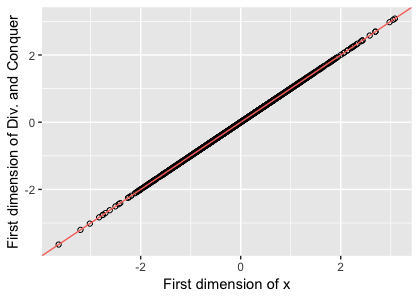
\includegraphics[width=4cm, height=4cm]{./images/first_div.png} }}%
    \qquad
    \subfloat[]{{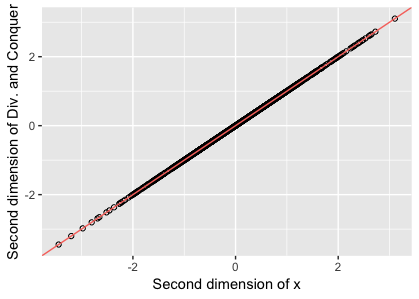
\includegraphics[width=4cm, height=4cm]{./images/second_div.png} }}%
    \qquad
    \subfloat[]{{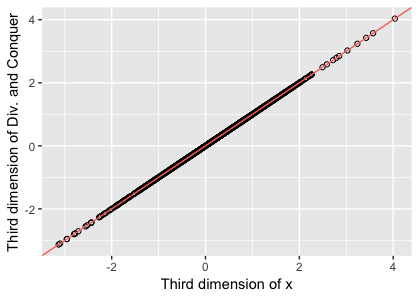
\includegraphics[width=4cm, height=4cm]{./images/third_div.png} }}
    \caption{Dimesion 1,2 and 3 of \textbf{X} against dimensions 1,2 and 3 of  $\mathbf{MDS_{Div}}$. \newline
            In red, the line $x=y$.}%
    \label{divide_example}%
\end{figure}


\begin{table}[ht]
\centering
\begin{tabular}{rrrr}
  \hline
 & 1 & 2 & 3 \\ 
  \hline
1 & 1 & 0.02 & -0.04 \\ 
  2 & 0.02 & 1 & 0.02 \\ 
  3 & -0.04 & 0.02 & 1 \\ 
   \hline
\end{tabular}
\caption{Correlation of \textbf{X} and $\mathbf{MDS_{Div}}$.} 
\label{corr_mds}
\end{table}



\section{Fast Multidimensional Scaling}
During the process of gathering information about work previously done around
MDS with big datasets, we found that \citeN{Yang06afast} already did an 
algorithm, they named it \textit{Fast Multidimensional Scaling}. 


\subsection{Algorithm}

\begin{itemize}

\item Divide \textbf{X} into $\mathbf{X_1},\dots, \mathbf{X_p}$.

\item Compute MDS for each $\mathbf{X_i}$: 
$\mathbf{MDS_1}, \dots, \mathbf{MDS_p}$. These individuals MDS solutions are 
stitched together by sampling $s$ points (rows) from each submatrix 
$\mathbf{X_i}$ and putting them into an alignment matrix 
$\mathbf{M_{align}}$ of size $sp \times sp$. In principle, $s$ should be at 
least 1 + the estimated dimensionality of the dataset. In practice, they 
oversample by a factor of 2 or more. 

\item MDS is run on $\mathbf{M_{align}}$. After this, it is obtained
$\mathbf{mMDS}$. Given a sampled point, there are two solutions of MDS: 
one from $\mathbf{X_i}$ and another one from $\mathbf{M_{align}}$.

\item The next step is to compute the Procrustes transformation to  line  
these two sets of solutions up in a common coordinate system:

\[
\mathbf{mMDS_i} = s_i \mathbf{dMDS_i} \mathbf{T_i} + \mathbf{1t_i}'
\]
where:

\begin{itemize}

\item $\mathbf{dMDS_i}$ is $\mathbf{MDS_i}$ but taking into account just
the subset of the sample points that belongs to partition $i$.

\item $\mathbf{mMDS_i}$ is $\mathbf{mMDS}$ but taking into account just
the subset of the sample points that belongs to partition $i$
\end{itemize}

\item After doing the previous part, we obtain a set of $p$ Procrustes 
parameters $(s_i, \mathbf{T_i},  \mathbf{t_i})$. So, the next step is to 
apply this set of parameters to each $\mathbf{MDS_i}$, i.e, 

\[
\mathbf{MDS_i}^a := s_i \mathbf{MDS_i} \mathbf{T_i} + \mathbf{1t_i'}.
\]

\item The last step is to join $\mathbf{MDS_1}^a, \dots,  \mathbf{MDS_p}^a$ 
all together, i.e, 
\[
\mathbf{MDS_X}:= \mathbf{MDS_1}^a \cup \cdots \cup \mathbf{MDS_p}^a.
\]

\end{itemize}

\indent They apply this process recursively until the size of $\mathbf{X_i}$ is
optimal to run MDS on. They find the stop condition as follows. Let 
$l \times l$ be the largest matrix that allow MDS to be executed efficiently. 
There are two issues that impact the performance of the algorithm: the size of 
each submatrix after subdivision and the number of submatrices, $p$, that are 
stitched together at each step. Ideally, the size of each submatrix after 
division should be as large as possible without exceeding $l$. By the same
token, the size of $\mathbf{M_{align}}$ should be bounded by $l$. The number of 
submatrices to be stitched together, $p$, should be the largest number such 
that $sp \leq l$.

\subsection{Some indicators about the goodness of fit}
As we have done in \autoref{chap:ind_div}, we present some visual results of
this algorithm. The data used is the same as in \autoref{chap:ind_div}. We
call $\mathbf{MDS_{Fast}}$ the result that provides the previous algorithm.

\indent Figure (\ref{fast_example}) shows that, for this particular case,
the algorithm captures quite well the dimesions of the original data, 
providing a high goodness of fit. In addition, dimesion $i$ of 
$\mathbf{MDS_{Fast}}$ fits perfectly the same dimesions $i$ of \textbf{X} and 
just this one, as we can see in Table (\ref{corr_fast}).


\begin{figure}[ht]
    \centering
    \subfloat[]{{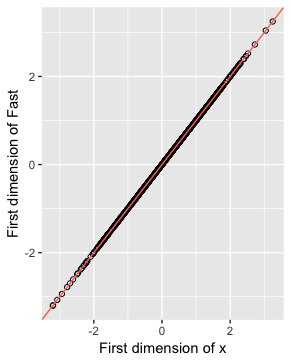
\includegraphics[width=4cm, height=4cm]{./images/first_fast.png} }}%
    \subfloat[]{{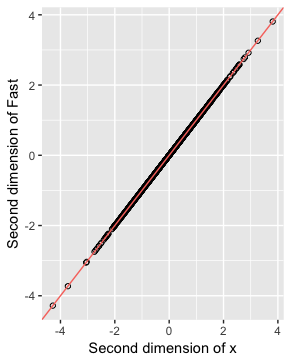
\includegraphics[width=4cm, height=4cm]{./images/second_fast.png} }}%
    \subfloat[]{{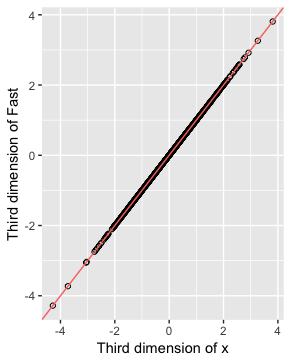
\includegraphics[width=4cm, height=4cm]{./images/third_fast.png} }}
    \caption{Dimesion 1,2 and 3 of \textbf{X} against dimensions 1,2 and 3 of  $\mathbf{MDS_{Fast}}$. \newline
            In red, the line $x=y$.}%
    \label{fast_example}%
\end{figure}


\begin{table}[ht]
\centering
\begin{tabular}{rrrr}
  \hline
 & 1 & 2 & 3 \\ 
  \hline
  1 & 1 & 0.02 & 0 \\ 
  2 & 0.02 & 1 & 0.02 \\ 
  3 & 0 & 0.02 & 1 \\ 
   \hline
\end{tabular}
\caption{Correlation of \textbf{X} and $\mathbf{MDS_{Fast}}$.} 
\label{corr_fast}
\end{table}

\section{Multidimensional Scaling based on Gower interpolation}

Gower interpolation formula \cite{gowerformula} allows to add a new set of 
points to a given MDS configuration. Given a matrix \textbf{X} $n \times p$, 
a MDS configuration for this matrix of dimension $n \times c$ and a matrix 
$\mathbf{X_{new}}$ $m \times p$, one wants to add these new $m$ 
rows to the existing MDS configuration. So, after adding this new rows, 
the MDS configuration will have $m+n$ rows and $c$ columns. 
We briefly summarise how to do so.

\begin{itemize}

\item Obtain $\mathbf{J} = \mathbf{I_n} - \frac{1}{n}\mathbf{1}\mathbf{1}'$,
where $\mathbf{I_n}$ is the identity matrix $n \times n$.

\item Given the distance matrix \textbf{D} of the rows of \textbf{X},
calculate $\mathbf{\Delta} = (\delta_{ij}^2)$.

\item Calculate $\mathbf{G} = - \frac{1}{2} \mathbf{J} \mathbf{\Delta} \mathbf{J}'$

\item Let \textbf{g} be the diagonal of \textbf{G}, i.e, 
$\mathbf{g} = \diag({\mathbf{G}})$.

\item Let \textbf{A} be the square distance matrix between the rows of 
\textbf{X} and the rows of $\mathbf{X_{new}}$. \textbf{A} has dimensions 
$m \times n$. Let $\mathbf{A}^2$ be the matrix of the square elements 
of \textbf{A}, i.e, $\mathbf{A}^2 = (a_{ij}^2)$.

\item Let \textbf{M} and \textbf{S} be the MDS for \textbf{X} and the 
variance-covariance matrix of the $c$ columns of \textbf{M}.

\item The MDS for the new $m$ observations is given by

\begin{equation} \label{gower_f}
\frac{1}{2n} (\mathbf{1}\mathbf{g} - \mathbf{A}^2) \mathbf{M}\mathbf{S}^{-1}.
\end{equation}

\end{itemize}

The resulting MDS for the $m$ observations of $\mathbf{X_{new}}$ is in the same
coordinate system as \textbf{M}. So, here it is not needed to do any 
Procrustes transformation.

\subsection{Algorithm}

\begin{itemize}
\item Divide \textbf{X} into $p$ partitions $\mathbf{X_1},\dots, \mathbf{X_p}$.

\item Calculate \textbf{J}, $\mathbf{\Delta}$, \textbf{G}, \textbf{g},
\textbf{A}, \textbf{M} and \textbf{S} according to the above formulas.

\item Obtain MDS for the first partition $\mathbf{X_1}$. 

\item Given a partition $1 < k \leq p$, do the following steps to get the 
related MDS:

\begin{itemize}

\item Calculate the distance matrix between the rows of $\mathbf{X_1}$ and
$\mathbf{X_k}$ and calculate the square of each element of this matrix. Let
$\mathbf{A}^2$ be this matrix (same as above).

\item Use Gower interpolation formula (\ref{gower_f}) to obtain MDS for 
partition $k$. 

\item Accumulate this solution.


\end{itemize}

\end{itemize}


As in the previous two algorithms, there is a key parameter to choose: $p$,
the number of partitions. For this algorithm, $p$ is set in the following way.
Let $l \times l$ be the largest distance matrix that a computer can calculate 
efficently. The value of $p$ is set as $n/p$.


\subsection{Some indicators about the goodness of fit}
We repeat the same as in \autoref{chap:ind_div}. Figure (\ref{gower_example}) 
and Table (\ref{corr_gower}) shows that the algorithm, for this particular case, 
captures quite well the dimesions of the original data, providing a high 
goodness of fit.

\begin{figure}[ht]
    \centering
    \subfloat[]{{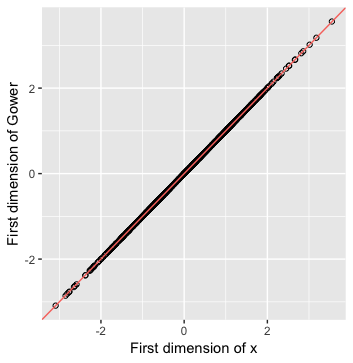
\includegraphics[width=4cm, height=4cm]{./images/first_gower.png} }}%
    \subfloat[]{{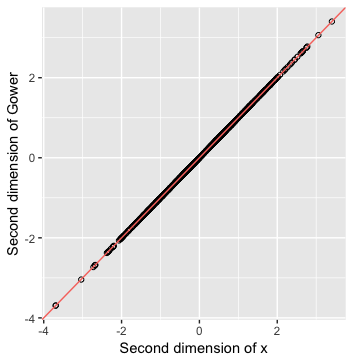
\includegraphics[width=4cm, height=4cm]{./images/second_gower.png} }}%
    \subfloat[]{{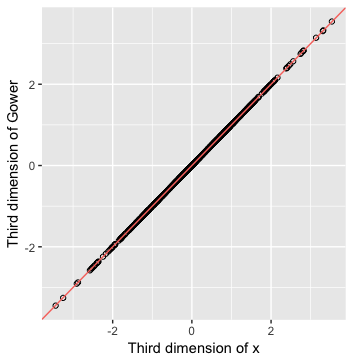
\includegraphics[width=4cm, height=4cm]{./images/third_gower.png} }}
    \caption{Dimesion 1,2 and 3 of \textbf{X} against dimensions 1,2 and 3 of  $\mathbf{MDS_{Gower}}$. \newline
            In red, the line $x=y$.}%
    \label{gower_example}%
\end{figure}


\begin{table}[ht]
\centering
\begin{tabular}{rrrr}
  \hline
 & 1 & 2 & 3 \\ 
  \hline
  1 & 1 & 0 & -0.04 \\ 
  2 & 0 & 1 & -0.0 \\ 
  3 & -0.04 & -0.03 & 1 \\ 
   \hline
\end{tabular}
\caption{Correlation of \textbf{X} and $\mathbf{MDS_{Gower}}$.} 
\label{corr_gower}
\end{table}


\section{Comparison of the algorithms}
\indent The three previous algorithms share the same goal: obtaining a MDS 
configuration for a given big dataset. However, there are some differences 
between the approaches that impact the performance of the algorithms. 
The main differences between them are:

\begin{itemize}
\item \textit{Divide and Conquer} uses a guide (the first subset, $\mathbf{X_1}$)
to align the solutions as well as it uses the whole partition $\mathbf{X_i}$ to
find the Procrustes parameters. However, \textit{Fast} does not use a guide an 
it uses a set of subsamples to find the Procrustes parameters.

\item \textit{Fast} is based on recursive programming. It divides until 
a manageable dimensionality is found. However, \textit{Divide and Conquer} 
estimates such a dimensionality.

\item \textit{MDS based on Gower interpolation} does not need any Procrustes
transformation. 

\end{itemize}

The fact that we found three algorithms to compute MDS arises some questions 
that need to be answered:

\begin{itemize}
\item Are these algorithms able to capture the data dimensionaly as good as 
calssical MDS does?
\item Which is the fastest method?
\item Can they deal with big datasets in a reasonable amount of time?
\item How are they performing when dealing with big data sets?
\end{itemize}

All these questions and are answered in \autoref{chap:sim}.

\section{Output of the algorithms}
The three algorithms have the same type of output. It consists on a list of 
two parameters. 

\indent The first parameter is the MDS calculated by the algorithm. It is a 
matrix of $n$ rows and $c$ columns, where $n$ is the number of rows of the 
input data and $c$ is the number of dimensions the user has required.

\indent The second paramenter is a list of eigenvalues. When performing MDS
a distance matrix is calculated and a singular value decomposition is performed
over this distance matrix. Each eigenvalue is divided by the number of 
observations taken into account to obtain the distance matrix. We refer to 
this as the \textit{normalized eigenvalues}. The previous list is 
returned.



\chapter{Simulation study}

\section{Design of the simulation}

\label{chap:sim}
Given the three algorithms, we would like to know how they are 
performing. There are two issues to study:

\begin{itemize}
\item Goodness of fit of the algorithms: are they able to capture data
dimensionality?
\item Performance in terms of time: are they `` fast" enough? Which one is 
the fastest?
\end{itemize}

To test the algorithm under different conditions, a simulation study has been
carried out. The scenarios are obtained as a combination of:

\begin{itemize}
\item \textit{Sample size}: we use different sample sizes, combining small
data sets and big ones. A total of six sample sizes are used, which are:
$10^3, 3\cdot 10^3, 5\cdot10^3, 10^4, 10^5, 10^6$.

\item \textit{Data dimensionls}: we generate a matrix with two different number 
of columns: 10, 100.

\item \textit{Main dimensions}: given the data matrix \textbf{X} $n \times k$,
it is postmultiplied by a diagonal matrix that contains $k$ values, 
$\lambda_1, \dots, \lambda_k$. The first values are much higher than the rest.
The idea of this is to see if the algorithms are able to capture the main
dimensions of the original dataset, i.e, the columns  with the highest variance. 
We set 5 combinations for this variable, which are:

\begin{itemize}
\item All the columns with the same values of $\lambda$: 
$\lambda_1 = \cdots = \lambda_k = 1$.

\item One main dimension with $\lambda_1 = 15$ and 
$\lambda_2 = \cdots = \lambda_k = 1$.

\item  Two main dimensions of the same value $\lambda$: 
$\lambda_1  = \lambda_2 = 15$, $\lambda_3 = \cdots \lambda_k = 1$.

\item  Two main dimensions of different values $\lambda$: 
$\lambda_1  = 15$, $\lambda_2 =10$, $\lambda_3 = \cdots \lambda_k = 1$.

\item  Four main dimensions of the same value $\lambda$: 
$\lambda_1  = \lambda_2 = \lambda_3 = \lambda_4 = 15$, $\lambda_5 = \cdots \lambda_k = 1$.


\end{itemize}

\item As distribution, it is a Normal one with $\mu = 0$ and 
$\sigma = 1$. With this distribution, we generate a matrix of $n$ observations
and $k$ columns, being the $k$ columns independent. After generating the 
dataset \textbf{X}, it is postmultiplied by the diagonal matrix that contains
de values of $\lambda$'s.


\end{itemize}

There is a total of 60 scenarios to simulate. Given a scenario, it is 
replicated 100 times. For every simulation, it is generated a dataset 
(according to the scenario), and all the algorithms are run using this dataset.
So, a total of 6000 simulations are carried out.

\indent Table (\ref{scenearios_sim}) shows the 
configuration of each scenario. Given a scenario, \textit{scenario\_id} 
identifes it. We refer a scenario by its \textit{scenario\_id}. 

\begin{longtable}{|r|r|r|r|l|} 
%\centering
%\begin{tabular}{rrrrl}
\hline
& scenario\_id & sample\_size & n\_dimensions & value\_primary\_dimensions \\ 
\hline
1 & 1 & 1000 & 10 & NULL \\ 
\hline
2 & 2 & 1000 & 100 & NULL \\ 
\hline
3 & 3 & 1000 & 10 & 15 \\ 
\hline
4 & 4 & 1000 & 100 & 15 \\ 
\hline
5 & 5 & 1000 & 10 & c(15, 15) \\ 
\hline
6 & 6 & 1000 & 100 & c(15, 15) \\ 
\hline
7 & 7 & 1000 & 10 & c(15, 10) \\ 
\hline
8 & 8 & 1000 & 100 & c(15, 10) \\ 
\hline
9 & 9 & 1000 & 10 & c(15, 15, 15, 15) \\ 
\hline
10 & 10 & 1000 & 100 & c(15, 15, 15, 15) \\ 
\hline
\hline
11 & 2000 & 3000 & 10 & NULL \\ 
\hline
12 & 2001 & 3000 & 100 & NULL \\ 
\hline
13 & 2002 & 3000 & 10 & 15 \\ 
\hline
14 & 2003 & 3000 & 100 & 15 \\ 
\hline
15 & 2004 & 3000 & 10 & c(15, 15) \\ 
\hline
16 & 2005 & 3000 & 100 & c(15, 15) \\ 
\hline
17 & 2006 & 3000 & 10 & c(15, 10) \\ 
\hline
18 & 2007 & 3000 & 100 & c(15, 10) \\ 
\hline
19 & 2008 & 3000 & 10 & c(15, 15, 15, 15) \\ 
\hline
20 & 2009 & 3000 & 100 & c(15, 15, 15, 15) \\ 
\hline
\hline
21 & 4000 & 5000 & 10 & NULL \\ 
\hline
22 & 4001 & 5000 & 100 & NULL \\ 
\hline
23 & 4002 & 5000 & 10 & 15 \\ 
\hline
24 & 4003 & 5000 & 100 & 15 \\ 
\hline
25 & 4004 & 5000 & 10 & c(15, 15) \\ 
\hline
26 & 4005 & 5000 & 100 & c(15, 15) \\ 
\hline
27 & 4006 & 5000 & 10 & c(15, 10) \\ 
\hline
28 & 4007 & 5000 & 100 & c(15, 10) \\ 
\hline
29 & 4008 & 5000 & 10 & c(15, 15, 15, 15) \\
\hline
30 & 4009 & 5000 & 100 & c(15, 15, 15, 15) \\ 
\hline
\hline
31 & 6000 & 10000 & 10 & NULL \\ 
\hline
32 & 6001 & 10000 & 100 & NULL \\ 
\hline
33 & 6002 & 10000 & 10 & 15 \\ 
\hline
34 & 6003 & 10000 & 100 & 15 \\ 
\hline
35 & 6004 & 10000 & 10 & c(15, 15) \\ 
\hline
36 & 6005 & 10000 & 100 & c(15, 15) \\ 
\hline
37 & 6006 & 10000 & 10 & c(15, 10) \\ 
\hline
38 & 6007 & 10000 & 100 & c(15, 10) \\ 
\hline
39 & 6008 & 10000 & 10 & c(15, 15, 15, 15) \\ 
\hline
40 & 6009 & 10000 & 100 & c(15, 15, 15, 15) \\ 
\hline
\hline
41 & 20000 & 100000 & 10 & NULL \\ 
\hline
42 & 20001 & 100000 & 100 & NULL \\ 
\hline
43 & 20002 & 100000 & 10 & 15 \\
\hline
44 & 20003 & 100000 & 100 & 15 \\ 
\hline
45 & 20004 & 100000 & 10 & c(15, 15) \\ 
\hline
46 & 20005 & 100000 & 100 & c(15, 15) \\ 
\hline
47 & 20006 & 100000 & 10 & c(15, 10) \\ 
\hline
48 & 20007 & 100000 & 100 & c(15, 10) \\ 
\hline
49 & 20008 & 100000 & 10 & c(15, 15, 15, 15) \\ 
\hline
50 & 20009 & 100000 & 100 & c(15, 15, 15, 15) \\ 
\hline
\hline
51 & 30000 & 1000000 & 10 & NULL \\ 
\hline
52 & 30001 & 1000000 & 100 & NULL \\ 
\hline
53 & 30002 & 1000000 & 10 & 15 \\ 
\hline
54 & 30003 & 1000000 & 100 & 15 \\ 
\hline
55 & 30004 & 1000000 & 10 & c(15, 15) \\ 
\hline
56 & 30005 & 1000000 & 100 & c(15, 15) \\ 
\hline
57 & 30006 & 1000000 & 10 & c(15, 10) \\ 
\hline
58 & 30007 & 1000000 & 100 & c(15, 10) \\ 
\hline
59 & 30008 & 1000000 & 10 & c(15, 15, 15, 15) \\ 
\hline
60 & 30009 & 1000000 & 100 & c(15, 15, 15, 15) \\ 
\hline
\caption{Scenarios simulated} 
\label{scenearios_sim}
\end{longtable}
%\end{table}

\indent Note that scenarios 1, 2, 2000, 2001, 4000, 4001, 6000, 6001, 20000,
20001, 30000, 30001 are pure noise. We refer ot them as \textit{noisy 
scenarios}.

\indent In order to test the goodness of fit and to check the time of the 
algorithms, some metrics are calculated.

\begin{itemize}
\item Goodness of fit:
\begin{itemize}


\item We get the correlation between the main dimensions of the data and the
main dimensions after applying the algorithms. We get just the diagonal, i.e,
the correlation between dimension $i$ of the data and the dimension $i$ of the
algorithm. 

\item We get the \textit{normalized eigenvalues}.
\end{itemize}

\item Time: Given an algorithm, the elapsed time to get the corresponding MDS
configuration is stored.

\end{itemize}

\indent We do it in this way because we want to check some hypothesis. We 
expect the three algorithms to behave ``correcty". By it, we mean that the
behavior should be the same as if classical MDS were run. Therefore, we 
expect that the correlation between the main dimensions of the data and the
main dimensions of the MDS of each algorithm to be close to 1.

\indent In addition, the variance of the original data should be captured. 
So, given the highest \textit{normalized eigenvalues}, we expect that 
its square root is approximately 15 or 10 when the scenarios are not the 
\textit{noisy scenrarios}. 

\indent For the time of the algorithms, we have done some tests and it seems 
that \textit{MDS based on Gower interpolation} seems to be the fastest.
So, it will be tested.


\indent Given a scenario, the steps that we have performed to calculate  and to
store all the data needed is:

\begin{enumerate}

\item Generate the data according to the scenario. 

\item Run \textit{divide and conquer} algorithm and get the time and the 
\textit{normalized eigenvalues}.

\item Align $\mathbf{MDS_{Div}}$ and \textbf{X} using Procrustes.

\item Get the correlation between the main dimensions of $\mathbf{MDS_{Div}}$ 
and \textbf{X}.

\item Run \textit{fast} algorithm and get the time and the 
\textit{normalized eigenvalues}.

\item Align $\mathbf{MDS_{Fast}}$ and \textbf{X} using Procrustes.

\item Get the correlation between the main dimensions of $\mathbf{MDS_{Fast}}$ 
and \textbf{X}.

\item Run \textit{MDS based on Gower interpolation} algorithm and get the 
time and the \textit{normalized eigenvalues}.

\item Align $\mathbf{MDS_{Gower}}$ and \textbf{X} using Procrustes.

\item Get the correlation between the main dimensions of $\mathbf{MDS_{Gower}}$ 
and \textbf{X}.

\end{enumerate}


\indent There are some important details related to the previous process that 
we have taken into account to make the simulator process faster. When runnig 
the algorithms, we ask for as many columns as the original data has, i.e $k$.

\indent For the \textit{normalized eigenvalues}, we just get 6 eigenvalues 
instead of the full list of eigenvalues (orherwise we would get $n$ 
eigenvalues). 

\indent For Procruster we dot not allow dilations, otherwise we would not
know if the distance is preserved. In addition, we do not use all the columns 
to do the alignment, we select the main dimensions. If there is not any
main dimension, i.e it is one of the \textit{noisy scenarios},we just select 5 
columns. 

\indent To avoid memory problems with the alignment when $n$ is greater or 
equal to $10^5$, Procrustes is done in the following way:

\begin{enumerate}

\item Create $p$ partitions of \textbf{X} and the result of a given MDS 
algorithm ($\mathbf{MDS_{alg}}$). Both set of partitios contains exctaly the
same observations.


\item For each partition get the Procrustes parameters without dilations.

\item Accumulate the paramenters iteration after iteration. So, at the end, 
we obtain $\mathbf{R} = \sum_{i = 1}^p \mathbf{R_i}$ and 
$\mathbf{t} = \sum_{i = 1}^p \mathbf{t_i}$.

\item $\mathbf{R} = \mathbf{R}/p$ and $\mathbf{t} = \mathbf{t}/p$.

\item Apply these parameters to $\mathbf{MDS_{alg}}$ so that 
\textbf{X} and $\mathbf{MDS_{alg}}$ are in the same coordinate system and
they can be compared.


\end{enumerate}

\indent The algorithms have as input values a set of variables. The input matrix 
is already explained, but there is another parameter that has been used during 
the description of the algorithms: $l$. The meaning of $l$ is a little bit 
different in each algorithm, but for simplicity we set this value
equals to 500.

\indent Finally, there is an extra ``parameter" to take into account: the 
machine used to do the simulations. Since a total of 6000 simulations are
performed and some of them include big datasets, we use 
\textit{Amazon Web Services} (AWS) to carry out the simulations. 
10 servers of he same type are used: \textit{c5n.4xlarge}. It 
has 16 cores and 42 GB of memory RAM. This kind of server is designed for 
applications like batch and log processing, distributed and or 
real-time analytics. 






\chapter{Conclusions}

%\bibliographystyle{unsrt}
\bibliographystyle{chicago}
\bibliography{bibliography.bib}


\appendix 

\chapter{Code}
\label{chap:code}

\chapter{Problems encountered during the development}
% Los paquetes de R que existen y sus limitaciones
% Para alinear las soluciones --> procrustes
% Lo complicado que me resulto implementar el fast

\end{document}




% To do:
%%% Mencionar a Roger
%%% En las conclusiones poner cuando es mejor usar una tecnica u otra. Por
%%% ejemplo, me imagino que Divide puede ir muy bien cuando las poblaciones son
%%% muy distintas, porque usa matrices grandes para alinear. Sin embargo, fast 
%%% solo usa submuestras
%%% En terminos de tiempo, que usarias: el de gower
%%% He usado enumerate en los algoritmos cuando los he descrito


%\subsection{Algorithm}
%\begin{algorithm}[H]
%  \SetAlgoLined
%  \SetKwInOut{Input}{input}
%  \SetKwInOut{Output}{output}
%   \Input{x: (matrix) a dataset. \newline 
%   l: (integer) the largest matrix dimension that allows MDS to be executed eficiently. \newline
%   s: (integer) the estimated dimensionality of the matrx.
%  }
%  \Output{
%    The output is a list of two elements: \newline
%    points: (matrix) MDS configuration. \newline
%    eigen: (vector) The eigenvalues. \newline
%  }
%  {$ls_positions = list()$} \Comment*[r]{This list will contain the positions of the rows per each partition}
%  {$list_eigenvalues = list()$} \Comment*[r]{This list will contain the eigenvalues}
%  {$i_eigen = 1$};
%  {$p = ceiling(2*nrow(x)/l)$} \Comment*[r]{Total partitions}
%  {$groups = sample(x = p, size = nrow(x), replace = TRUE)$}
%  groups = sort(groups)
%  \While{not at end of this document}{
%    read current\;
%    \eIf{understand}{
%      go to next section \Comment*[r]{Some comment}
%      current section becomes this one\;
%    }{
%      go back to the beginning of current section\;
%    }
%  }
%  \caption{How to write algorithms}
%\end{algorithm}
